At the backbone of all classical protocols described in Section \ref{section:protocols}, it lies the need to generate random uniform distributions of either qubit states, Bloch vectors or shared randomness in $\mathbb{R^3}$. In Figure \ref{fig:results_random_states}, we can see that applying random unitary transformations to zero qubit states leads to uniformly distributed random qubit pure states, which can later be transformed into random Bloch vectors or normalized random vectors in $\mathbb{R^3}$ as needed. These random states are also the seed to compute random POVMs with rank-1 projectors, as described in Section \ref{section:povm_generation}. Hence, once proven we have means to generate random states and rank-1 POVMs, we can address the measurement process. 
\begin{figure}[h]
\centering
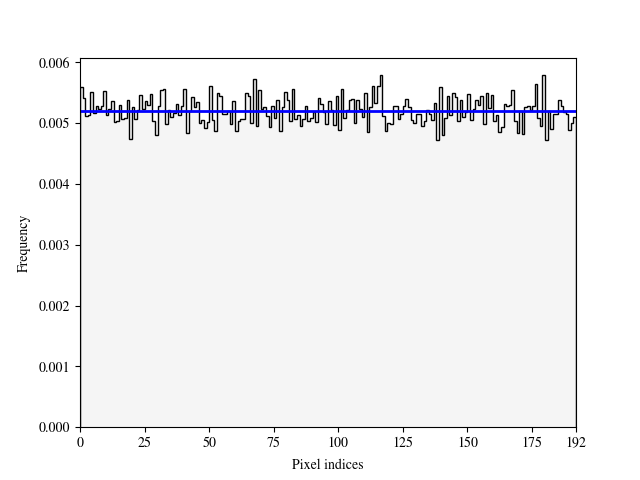
\includegraphics[width=\textwidth]{images/random_bloch_healpix.png}
\caption{In this histogram we see how the frequency distribution of $N=10^4$ random qubit states generated with \cite{software2023} follows a random uniform distribution of state vectors along the Bloch sphere (blue solid line). The frequencies are binned by HEALPix indices corresponding to an equal-area iso-latitude partition of the Bloch sphere with resolution $\mathit{NSIDE}=4$.}
\label{fig:results_random_states}
\end{figure}

The outcome probabilities for a given random POVM measure can be obtained analytically using the Born's rule, but we have gone a step further and used simulators and noisy intermediate-scale quantum computers (see Table \ref{table:quantum_resources}) to calculate such probabilities and compare them to the theoretical ones as described in \ref{section:quantum_circuit}. 
\newline
\begin{table}[h!]
\centering
\begin{tabular}{c c c c c} 
 \toprule
 Name & Qubits & Quantum Volume & CNOT Error & Readout Error \\ [1ex] 
 \midrule
 Nairobi & 7 & 32 & 0.01357 & 0.0227 \\ 
 Perth & 7 & 32 & 0.01733 & 0.0188 \\
 Oslo & 7 & 32 & 0.01 & 0.01667 \\
 Jakarta & 7 & 16 & 0.00773 & 0.0258 \\
 Lagos & 7 & 32 & 0.007243 & 0.0145 \\ 
 \bottomrule
\end{tabular}
\caption{Properties of Noisy Intermediate-Scale Quantum computers available at \href{https://quantum-computing.ibm.com}{IBM Quantum} to compute the prepare-and-measure outcome probabilities.}
\label{table:quantum_resources}
\end{table}

The quantum circuit resulting from applying Neumark's extension to a particular state and POVM measure is shown in Figure \ref{fig:quantum_circuit_example}. A summary of the achievable probability performances for such circuit using different quantum resources can be found in Table \ref{table:quantum_results}. Noisy quantum computers currently available to the public are limited to running circuits with a maximum of twenty thousand shots, so this results in less accuracy than desired. On the other hand, the Qiskit Aer simulator can perform noise-free simulations with a full range of shots, hence leading to better performances, as we will see later in the classical simulation results discussion. A full and comprehensive benchmark of IBM's free-access simulators and quantum computers for this prepare-and-measure scenario can be found in Appendix \ref{section:benchmark}.

\begin{figure}[!ht]
\centering
\begin{quantikz}
      \lstick{$\ket{\Psi}$}  & \gate[2][2cm]{U} & \meter{} \\
      \lstick{$\ket{0}$}  && \meter{} 
\end{quantikz}
\caption{Quantum circuit implementing a POVM measure of four elements. The unitary gate $U$ resulting from Neumark's is applied to the prepared state together with a single ancilla qubit such that the classical measurement leads to four possible outcomes: $\{00, 01, 10, 11\}$.}
\label{fig:quantum_circuit_example}
\end{figure}

A set of simulations have been conducted for the prepare-and-measure classical protocol using a random assortment of states and measurements, in addition to a collection of well-known measures like the Cross-POVM (\ref{eq:cross-povm}), the Trine-POVM (\ref{eq:trine-povm}) and a four-element SIC-POVM sample (\ref{eq:sic-povm}). 

\begin{landscape}
\topskip0pt
\vspace*{\fill}
\begin{tabular}{c|cccc|cccc|cccc}
\toprule
\textbf{Shots}  & \multicolumn{4}{c|}{$10^2$} 
                & \multicolumn{4}{c|}{$10^3$} 
                & \multicolumn{4}{c}{$2\cdot 10^4$}\\
\midrule
\textbf{Measure}  & 00 & 01 & 10 & 11
    & 00 & 01 & 10 & 11
    & 00 & 01 & 10 & 11\\
\midrule
Aer Simulator   & 0.370 & 0.150 & 0.070 & 0.410 
                & 0.362 & 0.117 & 0.067 & 0.454 
                & 0.378 & 0.120 & 0.058 & 0.443\\                
Nairobi         & 0.400 & 0.140 & 0.030 & 0.430 
                & 0.335 & 0.162 & 0.112 & 0.391 
                & 0.345 & 0.115 & 0.097 & 0.443\\               
Perth           & 0.350 & 0.260 & 0.100 & 0.290 
                & 0.337 & 0.185 & 0.121 & 0.357 
                & 0.328 & 0.152 & 0.113 & 0.408\\
Oslo            & 0.400 & 0.080 & 0.040 & 0.480 
                & 0.379 & 0.100 & 0.052 & 0.469 
                & 0.378 & 0.114 & 0.064 & 0.444\\
Jakarta         & 0.350 & 0.160 & 0.110 & 0.380 
                & 0.378 & 0.160 & 0.076 & 0.386 
                & 0.366 & 0.149 & 0.099 & 0.387\\   
Lagos           & 0.380 & 0.100 & 0.060 & 0.460 
                & 0.366 & 0.113 & 0.060 & 0.461 
                & 0.366 & 0.130 & 0.070 & 0.434\\
\midrule
\textbf{Born's rule}     & 0.375 & 0.125 & 0.064 & 0.435 
                & 0.375 & 0.125 & 0.064 & 0.435
                & 0.375 & 0.125 & 0.064 & 0.435\\
\bottomrule        
\end{tabular}
\captionof{table}{Example of probability distributions for circuit's classical measurement outcomes $\{00, 01, 10, 11\}$ obtained with different IBM Quantum systems and simulators. The prepare-and-measure scenario is that with state $\ket{\Psi}=\frac{3 + i \sqrt{3}}{4} \ket{0} - \frac{1}{2} \ket{1}$ and POVM measure $\mathbb{P}_4 = \{\frac{1}{2}\ket{0}\bra{0}, \frac{1}{2}\ket{1}\bra{1}, \frac{1}{2}\ket{+}\bra{+}, \frac{1}{2}\ket{-}\bra{-} \}$.}
\label{table:quantum_results}
\vspace*{\fill}
\end{landscape}

The results shown in Table \ref{table:classical_results_pm} clearly indicates that the correlations obtained by the classical prepare-and-measure simulations reproduce the quantum probabilities with extraordinary accuracy. The relative entropy distances among the theoretical probability distribution $P$, and the classical simulation probability distribution $Q$, on the sample space $\mathcal{X}$, have also been computed following the Kullback-Leibler divergence formula \cite{mackay2003}
\begin{equation}\label{eq:kullback}
D_{KL}(P||Q) = \sum_{x\in \mathcal{X}}{P(x)\ log\frac{P(x)}{Q(x)}}
\end{equation}
Figure \ref{fig:classical_results_kl} shows the Kullback-Leibler divergence among Born's rule and the classical simulation probabilities obtained for the set of prepare-and-measure scenarios in Table \ref{table:classical_results_pm}.
\newline
\begin{table}[h!]
\centering
{\renewcommand{\arraystretch}{1.5}%
\begin{tabular}{p{3cm}|c|cccc} 
 \toprule
 Scenario & Method & \multicolumn{4}{c}{Probabilities}  \\ \hline
 \multirow{2}*{Random-PVM$^1$} & Born & & & & \\ \cline{2-6}
 & {Simulation} & & & & \\ \hline
 \multirow{2}*{Cross-POVM$^2$} & Born & 0.3750 & 0.1250 & 0.0625 & 0.4375 \\ \cline{2-6}
 & Simulation & 0.3749 & 0.1250 & 0.0625 & 0.4376 \\ \hline
 \multirow{2}*{Trine-POVM$^3$} & Born &  &  &  &  \\ \cline{2-6}
 & Simulation &  &  &  &  \\ \hline
 \multirow{2}*{SIC-POVM$^4$} & Born & & & & \\ \cline{2-6}
 & Simulation &  &  &  &  \\ \hline
 \multirow{2}*{Random-POVM$^5$} & Born & & & & \\ \cline{2-6}
 & Simulation &  &  & &  \\ \hline
 \multirow{2}*{Random-POVM$^6$} & Born & & & & \\ \cline{2-6}
 & Simulation &  &  & & \\ 
 \bottomrule
\end{tabular}}
\caption{Probability outcomes of several prepare-and-measure classical simulations using a diverse set of measurements and prepared states $\ket{\Psi}$. The theoretical probabilities obtained applying Born's rule are also provided for ease of comparison. A total of  $10^7$ shots were used in the simulations.\\$^{1,2,3,4}\:\ket{\Psi}=\frac{3 + i \sqrt{3}}{4} \ket{0} - \frac{1}{2} \ket{1}$\\$^{5}\:\ket{\Psi}={x + iy } \ket{0} + {x + iy } \ket{1}$\\$^{6}\:\ket{\Psi}={x + iy } \ket{0} + {x + iy } \ket{1}$}
\label{table:classical_results_pm}
\end{table}

\begin{figure}[h!]
\centering
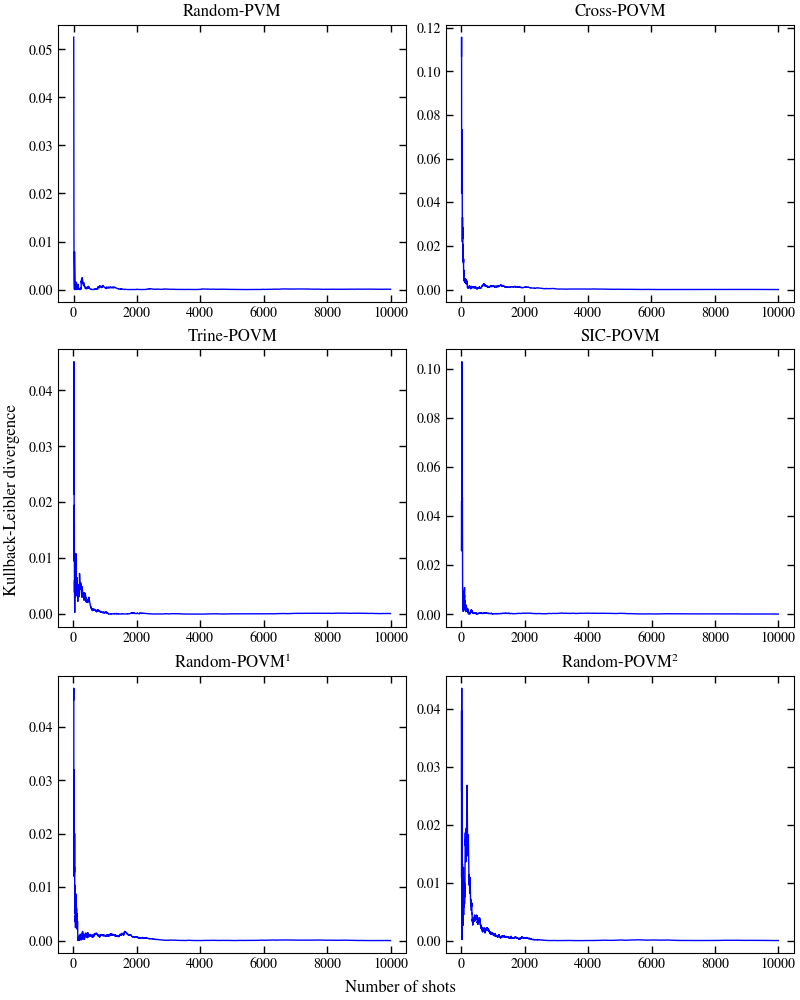
\includegraphics[width=\textwidth]{images/pm_povm_kl.png.png}
\caption{The Kullback-Leibler relative entropy among the theoretical probabilities and the simulation probability distributions for for the prepare-and-measure scenarios specified in Table \ref{table:classical_results_pm}. A total of $10^4$ shots were used for the simulations, and it can be clearly seen that the results converge to zero statistical distance rather quickly.}
\label{fig:classical_results_kl}
\end{figure}

Taking advantage of the analysis performed comparing theoretical and simulated probability distributions, we have extended the variational distance analysis to the prepare-and-measure scenario using IBM Quantum simulators. Figure shows that existing quantum simulators converge to the expected theoretical values slightly slower than the classical simulations. 

\begin{figure}[h!]
\centering
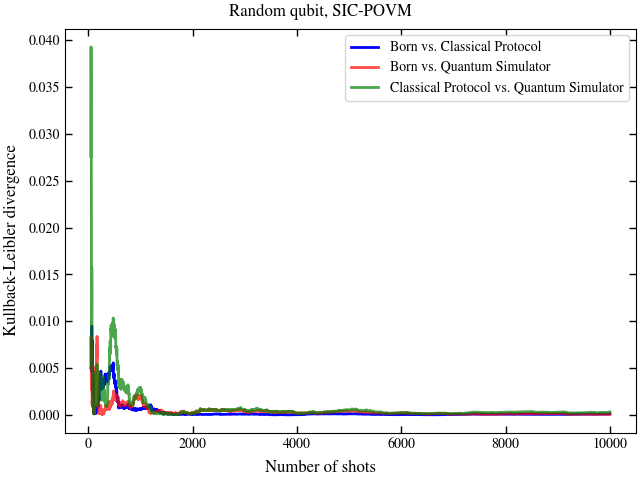
\includegraphics[width=0.7\textwidth]{images/pm_povm_kl_bcq.png}
\caption{The Kullback-Leibler relative entropy among the theoretical probabilities and the simulation probability distributions using the classical protocol and the IBM Quantum simulator. The prepared state selected is $\ket{\Psi}=3/4 + i \sqrt{3}/4 \ket{0} - 1/2 \ket{1}$, and the POVM measure the four-element SIC-POVM used in other examples (\ref{eq:sic-povm}). A total of $10^4$ shots were used for the simulations, where it can be noticed some differences in the convergence, particularly during the first thousands of runs.}
\label{fig:classical_results_kl}
\end{figure}